\documentclass[xcolor=table]{beamer}

\usepackage[serbianc]{babel}
\usepackage{graphicx}
\usepackage{makeidx}
\usepackage{listings}
\usepackage{adjustbox}
%\usepackage[table,xcdraw]{xcolor}

\lstset{
    escapechar={|},
}

\hypersetup{unicode}
\makeindex
\usefonttheme{professionalfonts}
\usetheme{CambridgeUS}

\title{System V File System}
\author{Борисав Живановић}

\begin{document}

    \begin{frame}
        \maketitle
    \end{frame}
    
    \begin{frame}{Шта рачунар заиста зна да ради?}
        \begin{itemize}
            \item Језик рачунара: \textbf{скуп инструкција} (енгл. ISA, Instruction Set Architecture)
            \item Аритметичке операције: \textbf{add}, \textbf{sub}, \textbf{div}, \textbf{mul}, …
            \item Померање података:
            \begin{itemize}
                \item са улазног уређаја у меморију
                \item из меморије на излазни уређај
                \item са једне меморијске локације на другу
            \end{itemize}
            \item Условно гранање: извршавање кода уколико је логички услов испуњен
        \end{itemize}
    \end{frame}
    
    \begin{frame}[allowframebreaks]{Меморијска хијерархија}
        \textit{
            Ideally one would desire an indefinitely large
            memory capacity such that any particular... word
            would be immediately available... We are... forced
            to recognize the possibility of constructing a
            hierarchy of memories each of which has greater
            capacity than the preceding but which is less
            quickly accessible.
        }

        \begin{flushright}
            \textbf{Burks, Goldstine, von Neumann} (1946)
        \end{flushright} 

        \framebreak
        
        \begin{itemize}
            \item Проблем: не постоји бесконачно брза и бесконачно велика меморија
            \item Чињеница: постоје технологије меморије које омогућавају релативно велики капацитет, по цену релативно мале брзине
            \begin{itemize}
                \item ...као и обрнуто!
                \item брзина и капацитет меморије су, по правилу, обрнуто сразмерни
            \end{itemize}
            \item Да ли је могуће добити највећи капацитет уз највећу брзину, по најмањој цени?
            \item Меморијска хијерархија нам ово \textit{донекле} омогућава
            \begin{itemize}
                \item цена: \textit{приближно} најспорија меморија
                \item брзина: \textit{приближно} најбржа меморија
            \end{itemize}
        \end{itemize}
        
        \framebreak

        \begin{figure}
            \centering
            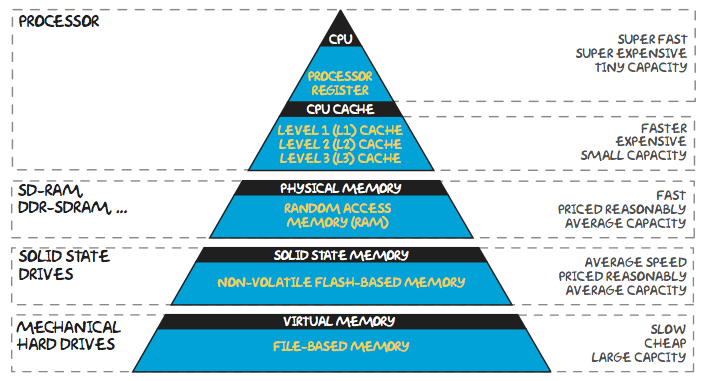
\includegraphics[width=\textwidth,height=0.7\textheight,keepaspectratio]{images/mem1.jpg}
            \label{fig:mem1}
        \end{figure}
    \end{frame}
    
    \begin{frame}{Контрола приступа у хардверу}
        \begin{itemize}
            \item Рачунар без контроле приступа би донекле био употребљив у једнокорисничком окружењу
            \begin{itemize}
                \item ...али неупотребљив у вишекорисничком
                \item чак и у једнокорисничком окружењу, одсуство изолације процеса представља велику опасност
            \end{itemize}
            \item Основне градивне блокове је неопходно имплементирати у хардверу
            \begin{itemize}
                \item софтвер можда неће бити рад да сарађује!
            \end{itemize}
            \item Кључни механизми: режими рада процесора, виртуелна меморија
        \end{itemize}
    \end{frame}
    
    \begin{frame}{Режими рада процесора}
        \begin{itemize}
            \item Привилеговани: IO, меморијске табеле, табеле прекида
            \begin{itemize}
                \item кернел
            \end{itemize}
            \item Неривилеговани: аритметичко/логичке операције, условно гранање, ограничен приступ меморији, системски позив
            \begin{itemize}
                \item кориснички софтвер
            \end{itemize}
            \item Прелазак из непривилегованог у привилеговани режим је могућ приликом прекида или системског позива
            \item Кернел одбија захтев уколико кориснички процес нема потребне привилегије и убија га
        \end{itemize}
    \end{frame}
    
    \begin{frame}[allowframebreaks]{Покретање оперативног система}
        \begin{itemize}
            \item Процесор се буди у привилегованом режиму
            \item Учитава се кернел
            \item Иницијализују се табеле прекида
            \item Иницијализују се меморијске табеле
            \item Контрола се предаје корисничким програмима, прелази се у непривилегован режим
            \item Овако подешен посредник (кернел) више није могуће уклонити или заобићи
            \begin{itemize}
                \item ...под претпоставком да нема багова у имплементацији кернела и хардвера
            \end{itemize}
        \end{itemize}
        
        \framebreak
        
        \begin{figure}
            \centering
            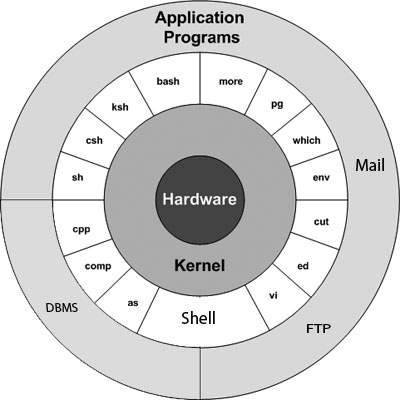
\includegraphics[width=\textwidth,height=0.8\textheight,keepaspectratio]{images/unix_architecture.jpg}
            \label{fig:unix_architecture.jpg}
        \end{figure}
    \end{frame}
    
    \begin{frame}{Литература}
        \begin{itemize}
            \item Operating Systems: Three Easy Pieces, Remzi H. Arpaci-Dusseau \& Andrea C. Arpaci-Dusseau
            \item Computer Organization and Design: The Hardware/Software Interface, David A. Patterson \& John L. Hennessy
            \item Системски софтвер (презентације), Иван Нејгебауер
            \item Operating Systems: Internals and Design Principles, William Stallings
            \item Preliminary Discussion of the Logical Design of an Electronic Computing Instrument
        \end{itemize}
    \end{frame}
\end{document}
